\documentclass[11pt]{article}

% ---- arXiv-safe preamble: standard TeX Live packages only ----
\usepackage[utf8]{inputenc}
\usepackage[T1]{fontenc}
\usepackage{lmodern}
\usepackage[margin=1in]{geometry}
\usepackage{graphicx}
\usepackage{booktabs}
\usepackage{amsmath,amssymb}
\usepackage{xcolor}
\usepackage{caption}
\usepackage{array}
\usepackage{microtype}
\usepackage{verbatim}
\usepackage[colorlinks=true,linkcolor=blue,citecolor=blue,urlcolor=blue]{hyperref}

\newcommand{\zbp}{ZeroBP-4B}
\captionsetup{font=small}
\setlength{\parskip}{0.4em}

\title{\bfseries ZeroBP at Scale and the Architecture of Capability:\\
A Boundary Study of a Backprop-Free 4B Language Model,\\ with a Trainable-Attention Control}
\author{Yanjin Li\\ \small Independent Research \\ \small \texttt{https://github.com/Yanjin-ai/zero-gradient}}
\date{2026}

\begin{document}
\maketitle

\begin{abstract}
\noindent This work studies, under a hard resource budget (a single T4 GPU, 3\,h), how far a
\emph{backprop-free} large language model can go, and---more importantly---\emph{why} it stops. The study
builds \zbp{}, a 4.16-billion-parameter content-routed mixture-of-experts (MoE) language model whose
entire training uses hand-written \textbf{local update rules} and \textbf{zero global backpropagation}
(no \texttt{autograd}), and locks it as a deterministic, reproducible submission
(WikiText-103 test perplexity $\approx 1391$ early-stop / $\approx 1355$ full-budget). On this fixed
backbone the study maps a \textbf{capability boundary} across three task structures that probe modern-LLM
competencies---bag-style sentiment, relational entailment (NLI), and multi-step modular arithmetic---under
increasing amounts of injected backpropagation (BP). The boundary is sharp and \emph{structural}: a little
embedding-path BP lifts sentiment from 60\% to 79\%, but neither a little nor a \emph{deep} BP installs
relational or multi-step structure at 4B (both stay at chance), and three ``ZeroBP-native'' routes each add
$\le 2$\,pp. A non-collapsing-readout probe shows the relational structure is \emph{not present anywhere} in
the frozen representation. To test whether these failures are properties of the \emph{tasks} or of the
\emph{architecture}, the study introduces a strictly isolated \textbf{architectural control} (the fifth and
final stage): a standard multi-layer trainable-attention Transformer trained with ordinary full backprop.
The same synthetic tasks that cap ZeroBP at 65.7\%/chance are solved to 100\% by a 0.8M-parameter control
model; on \textbf{real SNLI} the control backbone reaches \textbf{69.97\%} where \zbp{} is at chance
(33.4\%). The picture is reported plainly: the control backbone installs shallow multi-step reasoning
($k \le 3 = 100\%$) but hits its \emph{own} scale-resistant depth wall at $k \ge 4$; a from-scratch
character LM reaches only 2\% exact-match on real GSM8K; and \emph{neither} stack does real sentiment.
The result is a complete arc: \textbf{the ZeroBP relational/multi-step ceiling is architectural, not
fundamental---a trainable-attention backbone crosses it on real relational data and shallow multi-step
reasoning, while exposing new, honest limits of its own.}
\end{abstract}

\section{Introduction}

Modern large language models are trained with global backpropagation at enormous compute cost. Two
orthogonal questions motivate this work:
\begin{enumerate}
\item \textbf{How much language capability survives without global BP, under a strict single-GPU budget?}
Backprop-free / local-learning methods~\cite{hinton2022ff,lee2015difference} are attractive for memory- and
hardware-constrained settings, but their capability ceiling at scale is poorly characterized.
\item \textbf{When such a model fails a task, is the failure algorithmic (not enough gradient), architectural
(the backbone cannot represent the structure), or intrinsic to the task?} Disentangling these is usually
impossible because researchers change many things at once.
\end{enumerate}

This work approaches both with a deliberately layered study organized as \textbf{three lines}:
\begin{itemize}
\item \textbf{The submission line} (Section~\ref{sec:submission}): a pure-ZeroBP 4B MoE LM, engineered to be a
clean, deterministic, resource-budget baseline with \emph{zero} autograd anywhere in the training path.
\item \textbf{The boundary line} (Section~\ref{sec:boundary}): with that backbone \emph{frozen as an object
of study}, the study measures a task $\times$ method capability matrix, injecting increasing amounts of BP
into embeddings, attention, and blocks, and testing three ZeroBP-native structural levers.
\item \textbf{The control line} (Section~\ref{sec:control}): a strictly isolated control-backbone stack---a
standard trainable-attention Transformer with ordinary full BP---used as an architectural control to ask
whether the boundary of the second line is caused by the backbone.
\end{itemize}

These lines form a strict progression---each step is motivated by the result of the previous one, not run in
parallel. \textbf{Stage 1} establishes that a backprop-free model works at all. Only because it works does
\textbf{stage 2} ask where post-training succeeds and fails; only because reasoning fails does
\textbf{stage 3} try to remove the failure from inside the backbone; only because those fixes fail does
\textbf{stage 4} probe \emph{where} the missing structure lives. That diagnosis---the structure is absent
from the representation---yields a falsifiable hypothesis that the limit is \emph{architectural}, which
\textbf{stage 5} tests by swapping only the architecture. (The submission line is stage 1; the boundary line
spans stages 2--4; the control line is stage 5.) Figure~\ref{fig:arc} summarizes the arc.

The contribution is not a new state-of-the-art number. It is a \textbf{controlled boundary study}: a
reproducible backprop-free 4B baseline, a systematic capability matrix with a clean submission/research
isolation discipline, and an architectural control that turns ``ZeroBP can't do NLI'' into the sharper,
falsifiable claim ``\emph{this backbone} can't, and \emph{here is a backbone that can}, and \emph{here is
where even that one stops}.''

Three methodological commitments shaped the results: (i)~\textbf{fair readout}---capabilities are measured
with a fresh, task-agnostic readout head, because an unfair readout was found to fabricate or destroy
apparent capability (Sections~\ref{sec:probes},~\ref{sec:sst2}); (ii)~\textbf{single-lever changes}---each
experiment moves one structural degree of freedom; and (iii)~\textbf{honest correction}---two of the study's
hypotheses were refuted by later runs, and the corrections are reported rather than the original guesses.

\begin{figure}[t]
\centering
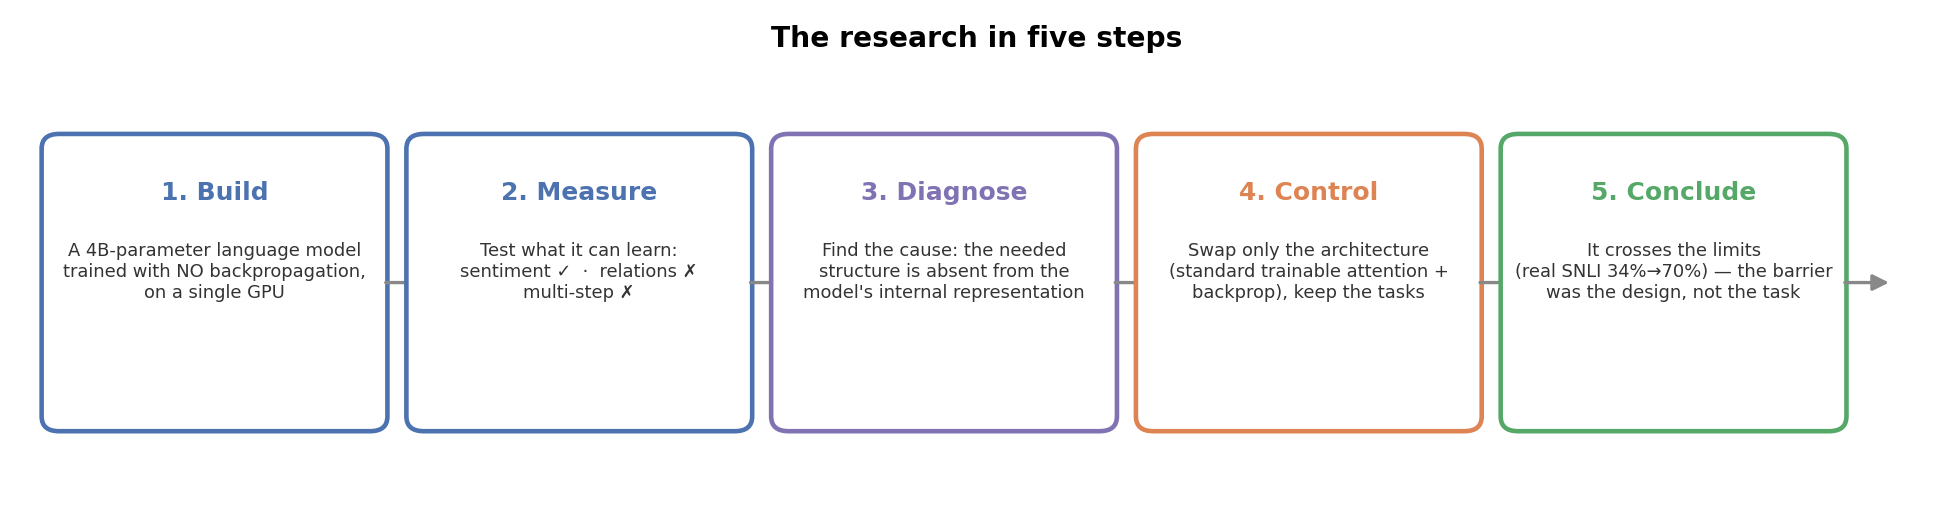
\includegraphics[width=\textwidth]{figures/research_arc.png}
\caption{The research in five stages. Each stage is driven by the result of the previous one.}
\label{fig:arc}
\end{figure}

\section{Related context}

The ZeroBP trainer sits in the family of \textbf{local-learning / backprop-alternative} methods (local
losses, target propagation~\cite{lee2015difference}, forward-only~\cite{hinton2022ff} and Hebbian-style
updates) and of \textbf{sparsely-activated MoE} models~\cite{shazeer2017moe,fedus2022switch}, but with an
unusual combination: a large resident expert bank whose experts are updated by hand-written local rules
under a deterministic sparse budget, with a frozen random attention ``reservoir''~\cite{jaeger2001esn}
feeding a last-position-collapsed representation into stacked routed blocks. The evaluation axes (LM
perplexity, sentiment, NLI, multi-step arithmetic / GSM8K, GLUE-SST2) are chosen to span the standard
capability dimensions used to characterize modern LLMs, at a scale where controlled ablation is affordable.
This work does not claim novelty of any single component; the contribution is the \textbf{boundary
methodology and the architectural control}.

\section{The submission line: a pure-ZeroBP 4B baseline}
\label{sec:submission}

\paragraph{Motivation and constraints.} The target environment is a single T4 (16\,GB) with a 3-hour wall
clock and self-supplied data---a setting in which standard BP training of a 4B model is infeasible
(measurements put a BP forward+backward of this model at ${\sim}31$\,GB, i.e.\ OOM). ZeroBP sidesteps the
backward pass entirely: there is no global loss gradient; every parameter update is a local rule.

\paragraph{Architecture and the zero-BP update.} \zbp{} is a decoder-style LM with the following data flow
(code-level fact):

{\small
\begin{verbatim}
token x  -->  E[x] + pos                          (embedding; |V|=32000, d=1024)
         -->  frozen random causal attention (Wq,Wk not trained)  (reservoir)
         -->  h = (emb + att*emb)[:, -1]      <-- last-position COLLAPSE: seq -> one [B,d]
         -->  4x stacked MoE block: content routing (EMA-prototype + capacity)
                  -> 950 experts, top-2
         -->  per-block deeply-supervised 2-layer-MLP readout head
                  + deterministic round-robin budget (k_update experts / block / step)
\end{verbatim}
}

\noindent with $d{=}1024$, $|V|{=}32000$, $\text{seq\_len}{=}64$, 4 layers, 950 experts/layer,
$k_{\text{route}}{=}2$, $k_{\text{update}}{=}4$, giving \textbf{4.160\,B fp16} resident parameters. Three
properties matter for the rest of the paper: (a)~\textbf{no global gradient}---training runs under
\texttt{set\_grad\_enabled(False)}, asserted by a gate; each expert is updated by a hand-written local rule
driven by the per-block deeply-supervised readout signal, and routing is a non-differentiable content
assignment (EMA prototypes + capacity); (b)~\textbf{deterministic sparse budget}---a round-robin schedule
updates only $k_{\text{update}}$ experts per block per step (0.42\% of the bank), which does not degrade LM
quality relative to dense updates ($k{=}1 \approx k{=}16$ in ablations) and bounds worst-case backlog (a
learned importance controller did \emph{not} beat this schedule and was rejected); (c)~\textbf{frozen
attention reservoir + last-position collapse}---the single attention layer is a frozen random reservoir
($W_q,W_k$ never trained), and the whole sequence is collapsed to the last position \emph{before} the routed
blocks. These two frozen choices become the prime suspects in Section~\ref{sec:boundary}.

\paragraph{Submission integrity.} A self-contained submission embeds the current trainer and runs the
default (pure-ZeroBP) path with no research flags. A gate suite asserts: resident params $\ge$ target,
\textbf{zero autograd}, monotone loss, val-ppl $<$ unigram, \textbf{determinism (re-run identical)}, and no
late drift. The submission file contains no \texttt{.backward} / \texttt{autograd.grad} / \texttt{enable\_grad}
and imports no research script; every research flag defaults to a no-op. The smoke config reproduces
$\text{final\_ppl}=6.251$ deterministically; the full 4B run fits the T4 at ${\sim}8.3$\,GB, ${\sim}8546$
tok/s.

\paragraph{Baseline.} With BPE subword tokenization + a 2-layer MLP readout head + a routing-freeze cosine
schedule, \zbp{} reaches \textbf{WikiText-103}~\cite{merity2017wikitext} test perplexity $\approx 1391$
(early stop, $t^{*} \approx 54$\,min) / $\approx 1355$ (full ${\sim}2.9$\,h budget), $\sim$51\% better than
the unigram baseline. \emph{(Erratum: a \texttt{load\_state\_dict} CPU-aliasing bug had contaminated some
multi-reset small-config runs; all small-config numbers below are corrected, and 4B/single-shot results were
unaffected---hence 4B confirmation is required before locking a claim.)}

\section{The boundary line: a ZeroBP capability matrix}
\label{sec:boundary}

Holding the backbone fixed, BP is injected only into embedding / attention / task-head parameters (never the
skeleton). All accuracies use a \textbf{fair readout}: a fresh closed-form (autograd-free) classification
head trained on the \emph{frozen} adapted representation, so what is measured is whether the
\emph{representation} gained structure rather than whether a BP head overfit.

\paragraph{Three task structures.} Sentiment (bag/compositional label); NLI (3-class relational entailment
requiring cross-clause alignment of \emph{two} entity pairs)~\cite{bowman2015snli}; 2-step arithmetic
(5-class sequential fold $((d_1 \circ d_2) \circ d_3) \bmod 5$).

\begin{table}[t]
\centering
\begin{tabular}{@{}llccc@{}}
\toprule
Task & Structure & 4B zero-shot & 4B little-BP & Small-config best \\
\midrule
Sentiment & bag composition & 60\% & \textbf{79\%} (emb.+head) & 100\% \\
NLI & relational alignment & 33.4\% (chance) & 33.4\% (no transfer) & $62\% \to 65.7\%$ (deep BP) \\
2-step arithmetic & multi-step compute & 24.7\% & ${\sim}19\text{--}21\%$ (chance) & ${\sim}$chance \\
\bottomrule
\end{tabular}
\caption{Task $\times$ method matrix (4B real + small-config cross-validation).}
\label{tab:matrix}
\end{table}

\paragraph{Findings.} \emph{Sentiment breaks} (Table~\ref{tab:matrix}): head-only reaches 59.9\% with zero
forgetting; a little embedding-path BP lifts it to \textbf{79\%} (at $+3.0$ ppl), and an ablation shows
\emph{embedding is the lever}. A measurement confound was traced here: an early ``57\%'' point used an
undertrained SGD readout head; the fair closed-form head corrected it to 79\%---a first sign that readout
choice can fabricate/hide capability. \emph{NLI does not transfer}: at 4B, zero-shot / emb-BP / emb+attn-BP
are \emph{all} chance, and a large-budget retry (3000 steps, high attention lr) is still chance.
\emph{Multi-step is uninstallable} at any BP component. Three \textbf{ZeroBP-native} levers barely move NLI:
richer data $+2.1$\,pp, structural auxiliary target $+0.5$\,pp, local attention rule $\approx 0$. A little
BP, by contrast, \emph{partially} installs it in the small config (fresh-head NLI $51.3 \to 58.8\%$ via
embedding, $\to 59.1\%$ adding attention), but the extra from attention is only $+0.3$\,pp and it does
\emph{not} transfer to 4B.

\subsection{Where is the relational structure?}
\label{sec:probes}

Three single-lever probes on the frozen/adapted backbone, each research-only and never touching the
submission:
\begin{itemize}
\item \textbf{Non-collapsing readout.} On the \emph{same frozen} base, replacing last-position collapse with
mean-pool / all-positions / concat does \emph{not} improve NLI---it drops (last-h 50.4\%, mean-pool 34.9\%
$\approx$ chance, all-positions 32.9\% $\approx$ chance). \textbf{The relational structure is not present
anywhere in the frozen representation}; a better readout cannot recover what is not there. This refuted the
``last-position collapse is the bottleneck'' hypothesis.
\item \textbf{Trainable attention, isolated.} Freezing the embedding and training \emph{only} $W_q,W_k$ on
the NLI loss gives $51.3 \to 51.3\%$ ($+0.0$\,pp), with verified weight movement
($\lVert \Delta W_q \rVert \approx 0.08$) and frozen embedding ($\lVert \Delta E \rVert = 0$). So the 59.1\%
of emb+attn is \emph{entirely embedding}; trainable attention \emph{in isolation} on this backbone is not a
lever. This refuted the ``trainable attention is the real lever'' hypothesis.
\item \textbf{Deeper BP.} Letting the MoE blocks train lifts small-config NLI to 65.7\%, but it does
\emph{not} transfer to 4B (NLI-4B remains chance), and arithmetic stays chance at every depth.
\end{itemize}

\paragraph{Boundary conclusion.} For bag tasks, ZeroBP + a little embedding BP is effective (79\%). For
\textbf{relational} (NLI) and \textbf{multi-step} (arithmetic) tasks, the \zbp{} architecture cannot install
the structure: it is absent from the representation, trainable attention in isolation adds nothing, and
multi-step is dead at every BP depth. The determinant is how much of a task lands in the embedding
(BP-installable) versus how much requires sequential computation through frozen blocks or cross-clause
attention alignment. Whether this is a property of the algorithm, the BP budget, or the \emph{backbone} is
answered by the control line.

\section{The control line: an isolated trainable-attention backbone}
\label{sec:control}

\paragraph{Design and isolation.} The control is a deliberately conventional pre-LN
Transformer~\cite{vaswani2017attention}: multi-head \emph{bidirectional} self-attention, GELU-MLP blocks,
residuals, and a \emph{non-collapsing mean-pool readout}, trained by ordinary full backprop (AdamW). It is
strictly isolated (pure code, zero dependency on the ZeroBP trainer; the submission never imports it and its
$6.251$/zero-autograd default is re-verified after every change). Evaluation uses the \emph{same} synthetic
distributions as Section~\ref{sec:boundary}, plus real SNLI, GSM8K~\cite{cobbe2021gsm8k}, and
SST-2~\cite{socher2013sst,wang2019glue}.

\begin{figure}[t]
\centering
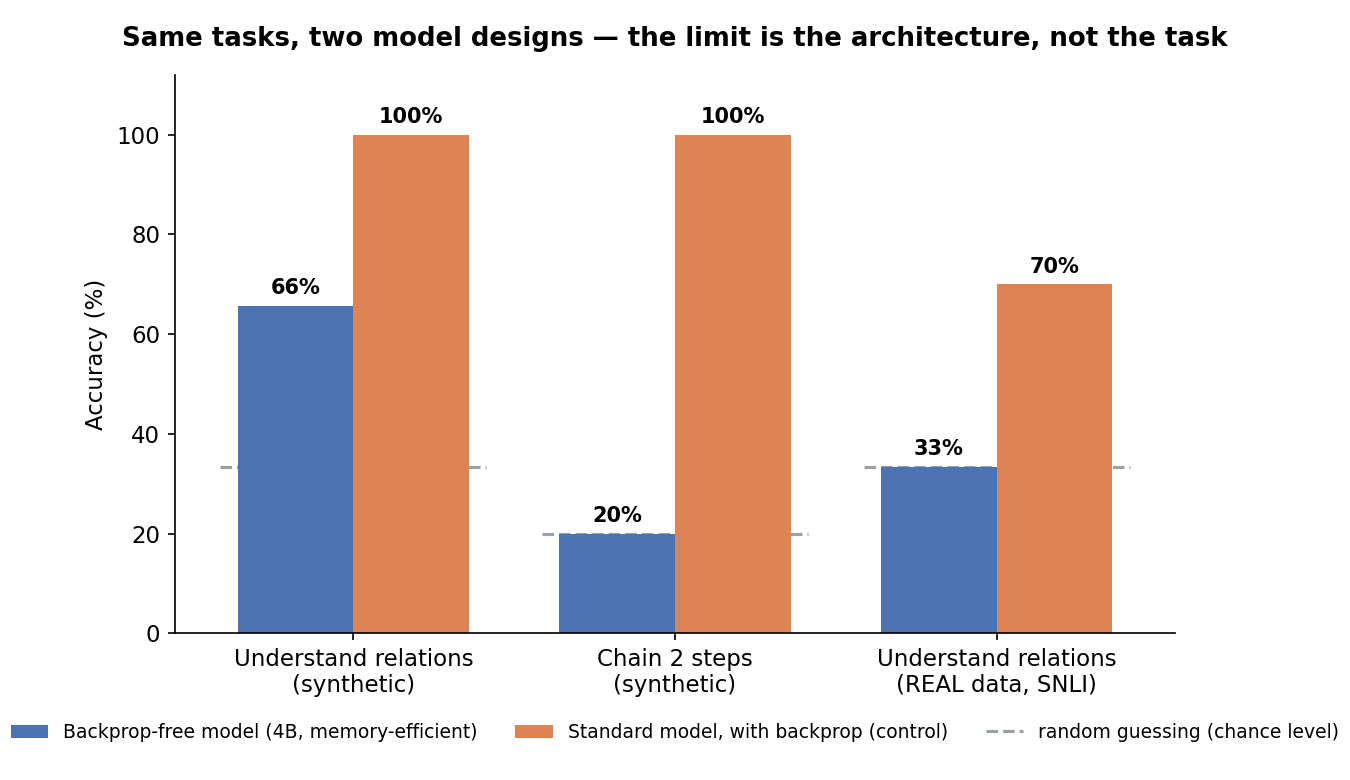
\includegraphics[width=0.92\textwidth]{figures/capability_comparison.png}
\caption{Same tasks, two designs. The backprop-free model cannot lift relational or multi-step tasks above
chance even with heavy tuning; a standard trainable-attention model solves them, including real SNLI.}
\label{fig:capability}
\end{figure}

\paragraph{G0: is the backbone the limit? (synthetic).} A 0.80M-parameter, 4-layer control model, full BP,
on the \emph{same} synthetic tasks:

\begin{table}[h]
\centering
\begin{tabular}{@{}lcc@{}}
\toprule
Task (synthetic, same dist.\ as Section~\ref{sec:boundary}) & Control backbone & \zbp{} / small \\
\midrule
NLI (3-class) & \textbf{100\%} @ step 500 & deep-BP 65.7\% (small) / chance (4B) \\
2-step arithmetic (5-class) & \textbf{100\%} @ step 1000 & chance at \emph{every} BP depth \\
\bottomrule
\end{tabular}
\caption{A 0.8M standard model installs both structures the ZeroBP backbone cannot---the boundary is
architectural, not task-intrinsic.}
\label{tab:g0}
\end{table}

\paragraph{G1: real relational data (SNLI).} A 12.4M-parameter (6-layer) control model on real SNLI (549k
train) reaches \textbf{val 69.97\%} (majority 33.8\%); \zbp{} on NLI is chance (33.4\%). The new backbone
reaches a modern small-LLM tier on a real relational benchmark that the ZeroBP stack structurally cannot
(Figure~\ref{fig:capability}). Because the control is a separate stack, this does not revise any ZeroBP
conclusion; it contextualizes it.

\paragraph{G2: how deep does multi-step go?} A per-depth sweep over the number of chained steps $k$, at two
scales (Table~\ref{tab:depth}, Figure~\ref{fig:wall}). The control installs \textbf{shallow multi-step}
($k \le 3 = 100\%$), decisively past ZeroBP (chance at \emph{any} depth, failing even $k{=}2$). But
$k \ge 4$ is a \textbf{wall}: $5\times$ the parameters and $2.5\times$ the steps moved it essentially nothing.
This refuted the ``under-capacity'' hypothesis. Formulation caveat: the task is direct answer-classification
with a mean-pool readout and \emph{no curriculum and no chain-of-thought}~\cite{wei2022cot}---the two
mechanisms most likely to break the wall, neither tested here.

\begin{table}[h]
\centering
\begin{tabular}{@{}lcc@{}}
\toprule
$n$ steps & 4.7M, 6k steps & deep: 21.3M, 15k steps \\
\midrule
$k=2$ & 100\% & 100\% \\
$k=3$ & 100\% (2.67M, local) & --- \\
$k=4$ & 22.5\% & 21.3\% \\
$k=6$ & 19.9\% & 19.8\% \\
$k=8$ & 20.6\% & 21.4\% \\
\bottomrule
\end{tabular}
\caption{Multi-step depth sweep (chance $=20\%$). $k \ge 4$ is scale-resistant.}
\label{tab:depth}
\end{table}

\begin{figure}[t]
\centering
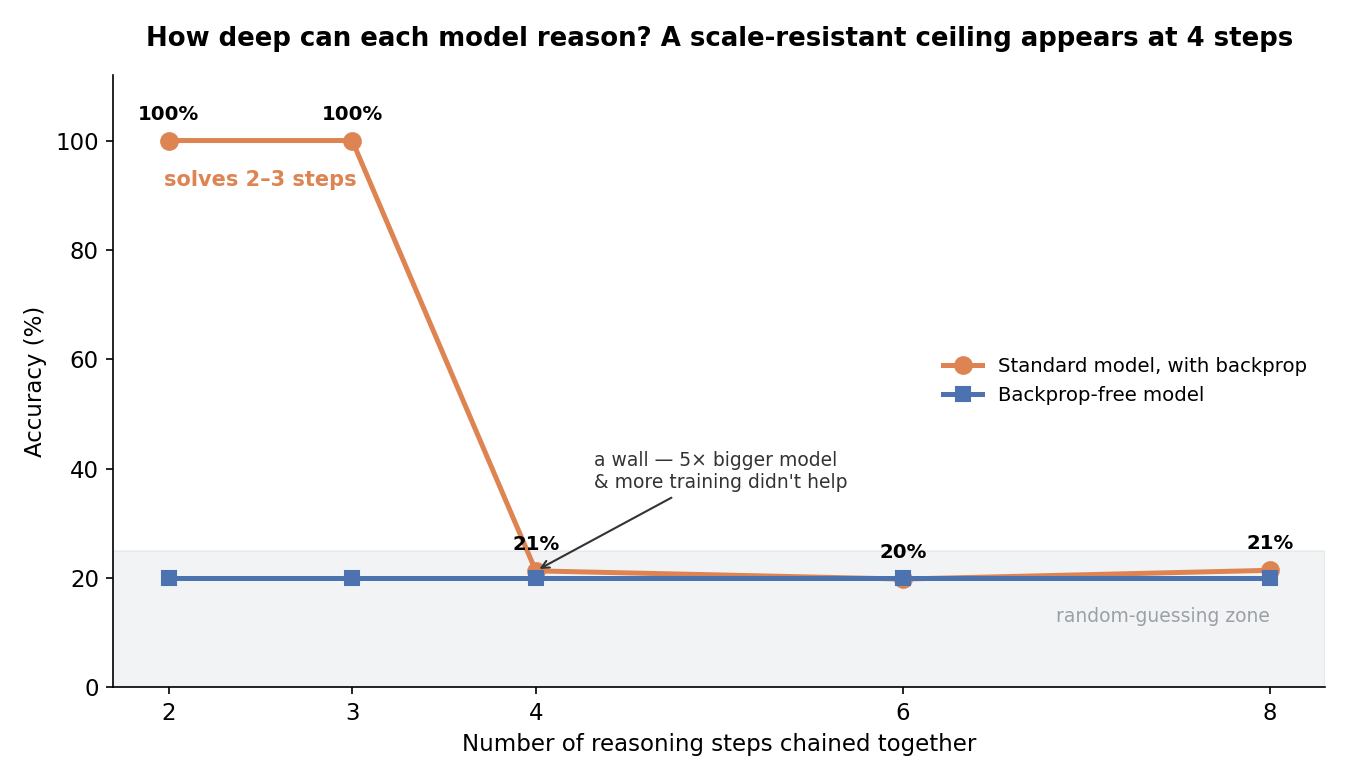
\includegraphics[width=0.92\textwidth]{figures/reasoning_depth_wall.png}
\caption{Reasoning-depth wall. The control solves 2--3 chained steps but stalls at $k \ge 4$, unchanged by a
$5\times$ larger model and longer training.}
\label{fig:wall}
\end{figure}

\subsection{Honest limits and a readout-collapse lesson}
\label{sec:sst2}

\paragraph{Generative GSM8K (stretch).} A 4.87M-parameter causal character LM, trained to \emph{generate} the
answer token-by-token and scored by exact-match, reaches \textbf{2.0\%} on real GSM8K (labeled a stretch in
advance; the synthetic generative smoke reached 66.6\%). It is reported plainly: the machinery works, the
model does not.

\paragraph{SST-2: a corrected negative.} The \zbp{} stack on real SST-2 first returned a bit-identical
49.08\% across zero-shot / emb-BP / emb+attn-BP. A diagnostic exposed the cause: the closed-form readout head
had \emph{collapsed} (predicting class-0 for all 872 examples), so 49.08\% was ``always negative,'' an
artifact. A fair BP linear probe (which uses both classes) reveals the truth:
$51.5\% \to 52.5\% \to 53.3\%$ (majority 50.9\%), i.e.\ $\approx$ chance. Real lexical sentiment is in the
same ``cannot install'' class as NLI/multi-step; the synthetic 79\% was an embedding-separable special case.
This is the second place a readout choice fabricated an apparent number, reinforcing the fair-readout
discipline.

\subsection{Final scorecard}

\begin{table}[h]
\centering
\begin{tabular}{@{}p{4.2cm}p{3.6cm}p{3.6cm}p{3.4cm}@{}}
\toprule
Dimension & Control backbone & \zbp{} (locked) & Conclusion \\
\midrule
Synthetic NLI + arithmetic & 100\% / 100\% & 65.7\% (small) / chance & backbone is the limit \\
Real SNLI & \textbf{69.97\%} & 33.4\% (chance) & relational structure installable \\
Multi-step depth & $k\le 3$=100\%, $k\ge 4$ wall & chance at any depth & new stack has its own ceiling \\
Generative GSM8K & EM ${\sim}2\%$ & --- & small-model stretch failure \\
Real SST-2 & --- & $\approx$ chance (probe 53\%) & real sentiment $\gg$ synthetic bag \\
\bottomrule
\end{tabular}
\caption{Capability scorecard (see also Figure~\ref{fig:scorecard}).}
\label{tab:scorecard}
\end{table}

\begin{figure}[t]
\centering
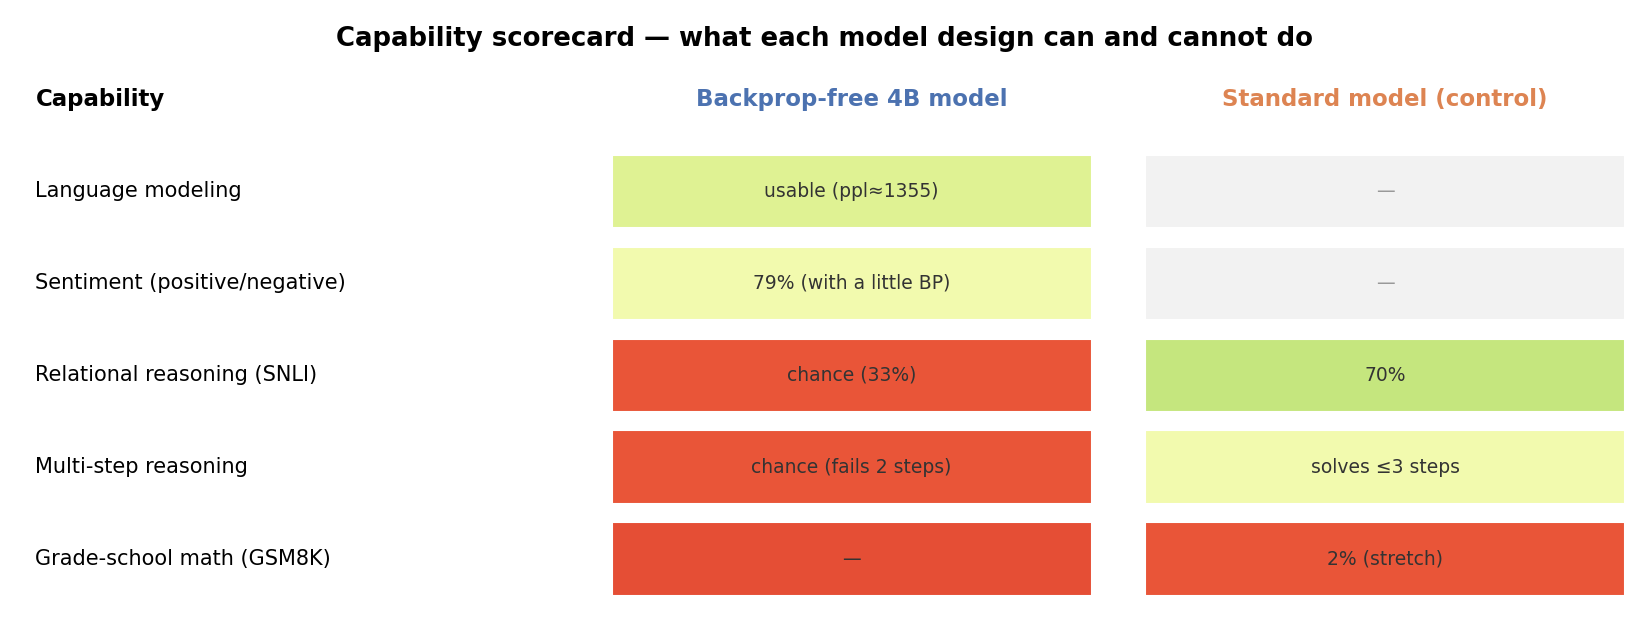
\includegraphics[width=0.95\textwidth]{figures/scorecard.png}
\caption{What each design can and cannot do. Green $=$ works, red $=$ fails/chance, grey $=$ not applicable.
Numbers are real measured results.}
\label{fig:scorecard}
\end{figure}

\section{Discussion: algorithm vs.\ architecture vs.\ task}

Because each factor was varied one at a time, three readings separate. \textbf{(i)~The \zbp{} ceiling is
architectural}: the relational structure is absent from the frozen representation
(Section~\ref{sec:probes}), trainable attention adds nothing in isolation, and multi-step is dead at any BP
depth; the prime suspects are the frozen attention reservoir (no cross-clause alignment can form) and the
last-position collapse (sequence structure discarded before the blocks). Embedding BP installs only what is
linearly composable at the token level---hence bag sentiment works and relational/sequential structure does
not. \textbf{(ii)~BP is necessary but not sufficient}: the same tasks are trivially installed by full BP on
a trainable-attention backbone, so gradient helps only where the architecture gives structure a trainable
place to live. This reframes ``ZeroBP can't do NLI'' as ``\emph{no} amount of BP into a
frozen-reservoir/last-collapse backbone installs relational structure; a standard attention backbone does so
easily.'' \textbf{(iii)~Task structure sets a consistent difficulty ordering} (bag $\ll$ relational $\ll$
multi-step-depth $\ll$ real generative math), and even a good backbone has honest limits: the control's
$k \ge 4$ wall is scale-resistant, suggesting deep sequential reasoning needs more than backbone $+$
scale---plausibly curriculum, intermediate supervision, or chain-of-thought~\cite{wei2022cot}.
\textbf{Methodologically}, two apparent numbers here were readout artifacts, not representation facts (an
undertrained SGD sentiment head; a collapsed SST-2 head)---capability claims about representations should use
a fair, task-agnostic probe, ideally two.

\section{Conclusion and future work}

\zbp{} is a reproducible, deterministic, backprop-free 4B LM that is genuinely useful under a single-T4
budget for LM and bag-style tasks (ppl $\approx 1355$--$1391$; sentiment 79\%) and serves as a controllable
object for measuring capability boundaries. Those boundaries are shown \emph{architectural} by an isolated
trainable-attention control that solves the same synthetic tasks (100\%), reaches 69.97\% on real SNLI, and
installs shallow multi-step---while exposing its own limits (a scale-resistant $k \ge 4$ wall, ${\sim}2\%$
GSM8K, near-chance real SST-2). \textbf{Future work:} break the $k \ge 4$ wall with curriculum /
chain-of-thought rather than raw scale; test advanced ZeroBP local rules on a \emph{trainable-attention}
substrate (combining the two lines); scale the control backbone (data $+$ parameters,
MNLI~\cite{williams2018mnli}/GSM8K) toward modern small-LLM behavior on relational/reasoning axes; and improve
ZeroBP LM quality while preserving zero-autograd purity.

\appendix
\section{Reproducibility and artifacts}
The submission (pure ZeroBP) is a single-source trainer whose default path asserts zero autograd and
reproduces $\text{final\_ppl}=6.251$ deterministically. The boundary line (research BP, isolated) and the
control line (\texttt{phase\_h/}) are separate scripts that the submission never imports. Every locked number
carries a commit hash in the experiment ledger; raw per-run result summaries accompany the code. Compute:
a single Kaggle T4 with concurrency capped at 2 GPU sessions. Repository:
\url{https://github.com/Yanjin-ai/zero-gradient}.

\section{Honest corrections log}
\begin{table}[h]
\centering
\begin{tabular}{@{}p{6.6cm}p{7.4cm}@{}}
\toprule
Claim as first stated & Correction \\
\midrule
Sentiment 4B $\approx$ 57\% (early point) & 79\% (undertrained SGD head $\to$ fair closed head) \\
``Last-position collapse is the bottleneck'' & Refuted: structure absent from the frozen rep at all positions \\
``Trainable attention is the real lever'' & Refuted: attention-only $+0.0$\,pp; embedding carries it \\
SST-2 (\zbp{}) $=$ 49\% flat & Readout-collapse artifact; true $\approx 53\%$ via fair BP probe \\
$k \ge 4$ multi-step is under-capacity & Refuted: $5\times$ params $+ 2.5\times$ steps unchanged $\to$ real wall \\
\bottomrule
\end{tabular}
\caption{Hypotheses refuted by later runs, retained transparently.}
\label{tab:corrections}
\end{table}

\begin{thebibliography}{99}
\bibitem{rumelhart1986} D.~E. Rumelhart, G.~E. Hinton, and R.~J. Williams. Learning representations by
back-propagating errors. \emph{Nature}, 323:533--536, 1986.
\bibitem{hinton2022ff} G.~E. Hinton. The Forward-Forward Algorithm: Some Preliminary Investigations.
\emph{arXiv:2212.13345}, 2022.
\bibitem{lee2015difference} D.-H. Lee, S.~Zhang, A.~Fischer, and Y.~Bengio. Difference Target Propagation.
In \emph{ECML-PKDD}, 2015.
\bibitem{jaeger2001esn} H.~Jaeger. The ``echo state'' approach to analysing and training recurrent neural
networks. \emph{GMD Technical Report 148}, 2001.
\bibitem{shazeer2017moe} N.~Shazeer, A.~Mirhoseini, K.~Maziarz, A.~Davis, Q.~Le, G.~Hinton, and J.~Dean.
Outrageously Large Neural Networks: The Sparsely-Gated Mixture-of-Experts Layer. In \emph{ICLR}, 2017.
\bibitem{fedus2022switch} W.~Fedus, B.~Zoph, and N.~Shazeer. Switch Transformers: Scaling to Trillion
Parameter Models with Simple and Efficient Sparsity. \emph{JMLR}, 23(120):1--39, 2022.
\bibitem{vaswani2017attention} A.~Vaswani, N.~Shazeer, N.~Parmar, J.~Uszkoreit, L.~Jones, A.~N. Gomez,
L.~Kaiser, and I.~Polosukhin. Attention Is All You Need. In \emph{NeurIPS}, 2017.
\bibitem{bowman2015snli} S.~R. Bowman, G.~Angeli, C.~Potts, and C.~D. Manning. A large annotated corpus for
learning natural language inference. In \emph{EMNLP}, 2015.
\bibitem{williams2018mnli} A.~Williams, N.~Nangia, and S.~R. Bowman. A Broad-Coverage Challenge Corpus for
Sentence Understanding through Inference. In \emph{NAACL}, 2018.
\bibitem{cobbe2021gsm8k} K.~Cobbe et al. Training Verifiers to Solve Math Word Problems.
\emph{arXiv:2110.14168}, 2021.
\bibitem{socher2013sst} R.~Socher, A.~Perelygin, J.~Wu, J.~Chuang, C.~D. Manning, A.~Ng, and C.~Potts.
Recursive Deep Models for Semantic Compositionality Over a Sentiment Treebank. In \emph{EMNLP}, 2013.
\bibitem{wang2019glue} A.~Wang, A.~Singh, J.~Michael, F.~Hill, O.~Levy, and S.~R. Bowman. GLUE: A Multi-Task
Benchmark and Analysis Platform for Natural Language Understanding. In \emph{ICLR}, 2019.
\bibitem{merity2017wikitext} S.~Merity, C.~Xiong, J.~Bradbury, and R.~Socher. Pointer Sentinel Mixture
Models. In \emph{ICLR}, 2017.
\bibitem{wei2022cot} J.~Wei, X.~Wang, D.~Schuurmans, M.~Bosma, B.~Ichter, F.~Xia, E.~Chi, Q.~Le, and
D.~Zhou. Chain-of-Thought Prompting Elicits Reasoning in Large Language Models. In \emph{NeurIPS}, 2022.
\end{thebibliography}

\end{document}
